\documentclass{beamer}
\usetheme{Padova}

\title{Conjunctive Disjunctive Node Kernel}

\author{Dinh Tran-Van$^1$, Alessandro Sperduti$^1$ and Fabrizio Costa$^2$ \\\vspace{.8em}
1- Department of Mathematics, University of Padova, Italy \\
2- Department of Computer Science, University of Exeter, UK \vspace{3em}}
\date{April $27^{th}$, 2017}

\begin{document}
\maketitle

\begin{frame}{Outline}
	\tableofcontents
\end{frame}


\section{Motivation}
%===================================
%===================================
%===================================
\begin{frame}[t]{Motivation}
\vspace{-.3cm}
\begin{block}{}
			\textbf{How to improve the performance of disease-gene association predictive systems?}
	\end{block}
\begin{columns}[T] % align columns
\begin{column}{.65\textwidth}
	\begin{itemize}
		\item Disease-gene association predictive systems are often based on the notion of relation between genes. \vspace{.3em}
		\item A common strategy is to encode gene-gene relations as a graphs and employ graph-based techniques to make inferences. \vspace{.3em}
		\item A key to determine the system's performance is the similarity measurement
	\end{itemize}
\end{column}%
%\hfill%
\begin{column}{.4\textwidth}
	\begin{figure}
	 \begin{flushright}% or better \raggedleft see comments below
	  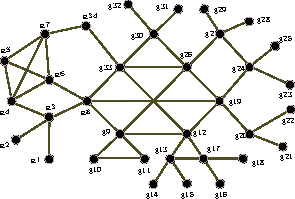
\includegraphics[width=1.0\textwidth, height=3.0cm]{images/example.pdf}
	  \caption{Genetic graph}
	 \end{flushright}
	\end{figure}

\end{column}%
\end{columns}
\end{frame}
%===================================
%===================================
%===================================
\begin{frame}[t]{Motivation}
\vspace{-.3cm}
\begin{block}{}
			\textbf{How to improve the performance of disease-gene association predictive systems?}
	\end{block}
\begin{columns}[T] % align columns
\begin{column}{.65\textwidth}
	\begin{itemize}
		\item Graph node kernels are normally used to measure node similarities. \vspace{.4em}
		\item Most node kernels are based on transitive properties and have limitations:\vspace{.4em}
		\begin{itemize}
			\item low discriminative capacity \vspace{.4em}
			\item prefering dense graphs, they show poor performances in case of sparse graphs.
		\end{itemize}
	\end{itemize}
\end{column}%
%\hfill%
\begin{column}{.4\textwidth}
	\begin{figure}
	  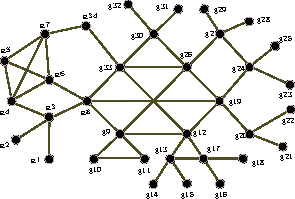
\includegraphics[width=1.0\textwidth, height=3.0cm]{images/example.pdf}
	  \caption{Genetic graph}
	\end{figure}

\end{column}%
\end{columns}
\end{frame}
%===================================
%===================================
%===================================
\begin{frame}[t]{Method}
\vspace{-.3cm}
\begin{block}{Proposed kernel}
	We propose Conjunctive Disjunctive Node Kernel (CDNK) which is an instance of decompositional graph kernel (DGK) [1] and a modification of NSPDK kernel [2].
\end{block} \vspace{.5em}

\begin{block}{Advantages}
	\begin{itemize}
		\item It takes advantage from NSPDK kernel which can explicitly model the configuration of nodes' context.\vspace{.4em}
		\item It contains a decompsition procedure which transforms graph into a collection of linked sparse subgraphs so that DGK can efficiently work. Therefore, we can use take dense or sparse graphs as the input of our kernel.
	\end{itemize}
\end{block}
	



\end{frame}
%===================================
%===================================
%===================================
\section{Method}

\begin{frame}[t]{Method}
	\begin{block}{Notations}
		\begin{itemize}
			\item $G = (V, E)$: an undirected, labeled graph with node set $V(E)$, and edge set $E(G)$ \vspace{.5em}
			\item $\mathcal{D}(u,v)$: shorest distance between $u$ and $v$ \vspace{.5em}
			\item $N_r(v) = \lbrace u|\mathcal{D}(v,u)\leq r \rbrace$: neighborhood set with radius $r$ \vspace{.5em}
			\item $\mathcal{N}_r^v$: subgraph formed by nodes and edges with endpoints in $N_r(v)$
		\end{itemize}
	\end{block}
\end{frame}
%===================================
%===================================
%===================================
\begin{frame}{Method}
	\begin{block}{Neighborhood Subgraph Pairwise Distance Kernel (NSPDK)}
\begin{itemize}
	\item NSPDK is an instance of decompositional kernels
	\item $R_{r,d}(A_u, B_v, G)$ is true if $A_u \cong N_r^u$, $B_v \cong N_r^v$ and $\mathcal{D}(u,v) = d$
	\item $R_{r,d}^{-1}(A_u, B_v, G) = \lbrace A_u, B_v | R_{r,d}(A_u, B_v, G) = true \rbrace$
	\item $\kappa_{r,d}(G,G^{'}) = 
\!\!\!\!\!\!\!\!\!\!\!\! 
\sum\limits_{\substack{A_u, B_v \ \in \ R_{r,d}^{-1}(G) \\ 
{A'}_{u'}, {B'}_{v'} \ \in \ R_{r,d}^{-1}(G')
}} \!\!\!\!\!\!\!\!\!\!\!\!  { { \textbf{1}_{A_{u} \cong A'_{u'}}} \cdot {
\textbf{1}_{B_{v} \cong B'_{v'}}} }$, where $\textbf{1}_{A \cong B}$ is the \textit{exact matching function} that returns 1 if $A$ is isomorphic to $B$ and 0 otherwise.
	\item $K(G,G') = \sum\limits_{r}{\sum\limits_{d}{\kappa_{r,d}(G,G')}}$ \\for efficiency reasons, the values of $r$ and $d$ are upper bounded to a given $r^*$ and $d^*$, respectively.
\end{itemize}		
	\end{block}
\end{frame}
%===================================
%===================================
%===================================
\begin{frame}[t]{Method}
	\begin{block}{Node Labeling}
We propose to use discretized functional annotation based on gene ontology. \vspace{.3em}
\begin{itemize}
	\item Each gene is representated as a vector of go-terms \vspace{.2em}
	\item Cluster genes into a given number of clusters \vspace{.2em}
	\item Genes are labeled as their cluster class identifiers \vspace{.2em}
\end{itemize}		
	\end{block}
\end{frame}
%===================================
%===================================
%===================================
\begin{frame}[t]{Method}
	\begin{block}{Node Labeling}
We propose to use discretized functional annotation based on gene ontology. \vspace{.2em}
\begin{itemize}
	\item Each gene is representated as a vector of go-terms \vspace{.2em}
	\item Cluster genes into a given number of clusters \vspace{.2em}
	\item Genes are labeled as their cluster class identifiers \vspace{.2em}
\end{itemize}		
	\end{block}
	\begin{block}{Graph Decomposition}
Transforming graph in a collection of linked sparse sub-graphs in which we use two types of links: \textit{conjunctive} and \textit{disjunctive}.
	\begin{itemize}
		\item \textit{conjunctive:} used for considering distance between nodes
		\item \textit{disjunctive:} used for connecting sparse subgraphs
	\end{itemize}
	\end{block}
\end{frame}
%===================================
%===================================
%===================================
\begin{frame}[t]{Method}
\vspace{-1cm}
\begin{columns}[t] % align columns
\begin{column}[t]{.5\textwidth}
	\begin{figure}
	  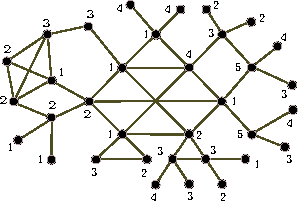
\includegraphics[width=1.0\textwidth, height=3.0cm]{images/Decomposition_0.pdf}
	\end{figure} 
	\textbf{$\bullet$ Iterative Kcore}: form a collection of linked subgraphs \vspace{.5em}\\
	\textbf{$\bullet$ Clique Decomposition}: similarly treat nodes belong same clique \vspace{.5em}\\ 
	
\end{column}%
%\hfill%
\begin{column}{.5\textwidth}


\end{column}%
\end{columns}
\end{frame}
%===================================
%===================================
%===================================
\begin{frame}[t]{Method}
\vspace{-1cm}
\begin{columns}[t] % align columns
\begin{column}[t]{.5\textwidth}
	\begin{figure}
	  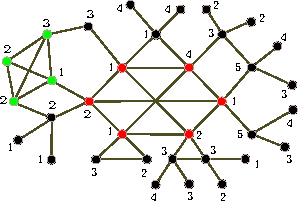
\includegraphics[width=1.0\textwidth, height=3.0cm]{images/Decomposition_1.pdf}
	\end{figure} 

	\textbf{$\bullet$ Iterative Kcore}: form a collection of linked subgraphs \vspace{.5em}\\
	\textbf{$\bullet$ Clique Decomposition}: similarly treat nodes belong same clique \vspace{.5em}\\ 
	
\end{column}%
%\hfill%
\begin{column}{.5\textwidth}

\end{column}%
\end{columns}
\end{frame}

%===================================
%===================================
%===================================
\begin{frame}[t]{Method}
\vspace{-1cm}
\begin{columns}[t] % align columns
\begin{column}[t]{.5\textwidth}
	\begin{figure}
	  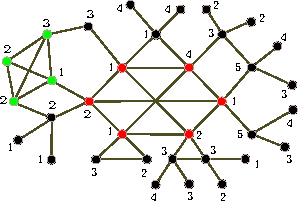
\includegraphics[width=1.0\textwidth, height=3.0cm]{images/Decomposition_1.pdf}
	\end{figure} 
	
	\textbf{$\bullet$ Iterative Kcore}: form a collection of linked subgraphs \vspace{.5em}\\
	\textbf{$\bullet$ Clique Decomposition}: similarly treat nodes belong same clique \vspace{.5em}\\ 
	
\end{column}%
%\hfill%
\begin{column}{.5\textwidth}
	\begin{figure}
	  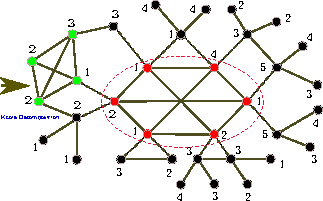
\includegraphics[width=1.0\textwidth, height=3.0cm]{images/Kcore.pdf}
	\end{figure}


\end{column}%
\end{columns}
\end{frame}
%===================================
%===================================
%===================================
\begin{frame}[t]{Method}
\vspace{-1cm}
\begin{columns}[t] % align columns
\begin{column}[t]{.5\textwidth}
	\begin{figure}
	  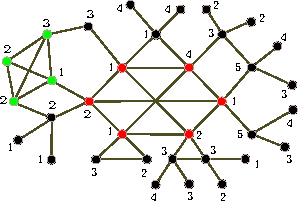
\includegraphics[width=1.0\textwidth, height=3.0cm]{images/Decomposition_1.pdf}
	\end{figure} 
	
	\textbf{$\bullet$ Iterative Kcore}: form a collection of linked subgraphs \vspace{.5em}\\
	\textbf{$\bullet$ Clique Decomposition}: similarly treat nodes belong same clique \vspace{.5em}\\ 
	
\end{column}%
%\hfill%
\begin{column}{.5\textwidth}
	\begin{figure}
	  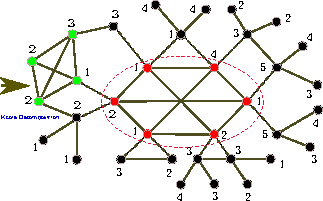
\includegraphics[width=1.0\textwidth, height=3.0cm]{images/Kcore.pdf}
	\end{figure}

	\begin{figure} \vspace{-.8cm}
	  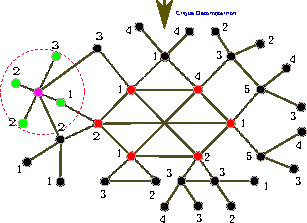
\includegraphics[width=1.0\textwidth, height=3.0cm]{images/Clique.pdf}
	\end{figure}

\end{column}%
\end{columns}
\end{frame}
%===================================
%===================================
%===================================

\begin{frame}{Method}
We first define:
\begin{itemize}
	\item Conjunctive relation: $R_{r,d}^\wedge(A_u, B_v, G_u)$ is true if $A_u \cong N_r^u$, $B_v \cong N_r^v$ and $\mathcal{D}(u,v) = d$ \vspace{.3em}
	\item Disjunctive relation: $R_{r,d}^\vee(A_u, B_v, G_u)$ is true if $A_u \cong N_r^u$, $B_v \cong N_r^v$ and $\mathcal{D}(w,v) = d$, $(u,w)$ is a disjunctive edge. \vspace{.3em}
	\item  $\kappa_{r,d}(G_u,G_{u'}) = \!\!\!\!\!\!\!\!\!\!\!\!
 \sum\limits_{\substack {A_u,{B}_{v} \in {R_{r,d}^{\wedge}}^{ -1}(G_u) \\ A'_{u'},{B'}_{v'} \in {R_{r,d}^{\wedge}}^{ -1}(G_{u'}) }} \!\!\!\!\!\!\!\!\!\!\!\!
  { \textbf{1}_{A_u \cong A'_{u'}} \cdot { \textbf{1}_{B_{v} \cong B'_{v'}}}}
+ \!\!\!\!\!\!\!\!\!\!\!\!
 \sum\limits_{\substack {A_u,{B}_{v} \in {R_{r,d}^{\vee}}^{ -1}(G_u) \\
  A'_{u'},{B'}_{v'} \in \ {R_{r,d}^{\vee}}^{ -1}(G_{u'}) }} \!\!\!\!\!\!\!\!\!\!\!\!
  { \textbf{1}_{A_u \cong A'_{u'}} \cdot { \textbf{1}_{B_{v} \cong B'_{v'}}}}
  $.
\end{itemize}
CDNK is defined as:
$K(G_u,G_v) = \sum\limits_{r}{\sum\limits_{d}{\kappa_{r,d}(G_u,G_v)}}$.

\end{frame}

\section{Empirical Evaluation}
\vspace{-1cm}
%\small
\begin{frame}[t]{Evaluation}
\small
We evaluate performance of kernels by employing gene prioritization on 12 diseases and using two datasets (followed [3]).
\begin{itemize}
	\item \textbf{Kernels}: K1: Diffusion kernel [4], K2: Markov difussion kerel [5], K3: Markov exponential diffusion kernel [3], K4: Regularized Laplacian kernel [6], K5: CDNK.
	\item \textbf{Datasets}: \textit{BioGPS} - a gene co-expression network (7311 nodes, 911,294 edges), and \textit{Pathways} - encode gene common pathway relations (7311 nodes, 2,254,822 edges). 
\end{itemize}

\textit{Table 1: Performance of kernels in term of average AUC and order ranking over all diseases}
\begin{center}
\setlength{\tabcolsep}{1mm}
\begin{tabular}{|c|c|c|c|c|c|c|c|c|c|c|c|}
	\hline 
		& \multicolumn{5}{c|}{\textbf{BioGPS}} & \multicolumn{5}{|c|}{\textbf{Pathways}} \\
	\hline
	Kenels & K1 & K2 & K3 & K4 & K5 & K1 & K2 & K3 & K4 & K5 \\ [0.6ex]
	\hline 
	$\overline{AUC}$ & 66.6 & 63.5 & 67.8 & 67.5 & \color{red}{73.3} & 62.7 & 70.1 & 75.3 & 75.5 & \color{red}{76.5} \\ [0.8ex]
	\hline
	$\overline{Rank}$ & 3.5 & 4.3 & 2.8 & 2.5 & \color{red}{2.0} & 4.8 & 3.9 & 2.5 & 2.0 & \color{red}{1.8} \\
	\hline 
\end{tabular}
\end{center}
\end{frame}
%===================================
%===================================
%===================================
\section{Conclusion}
\normalsize
	\begin{frame}{Conclusion}
	We have proposed Conjunctive Disjuctive graph node kernel that: \vspace{.4em}
	\begin{itemize}
		\item efficently exploit graph structure to form high discriminative node similarity measurement \vspace{.4em}
		\item includes a decomposition procedure which allows it to process with both sparse and dense graphs \vspace{.4em}
		\item shows state of the art performance
	\end{itemize}
	\end{frame}
%===================================
%===================================
%===================================		
\small
\begin{frame}{Reference }
\textit{1. Haussler, D. Convolution kernels on discrete structures. Technical report,
Department of Computer Science, University of California at Santa Cruz, 1999. \\
2. Fabrizio C., et al, Fast neighborhood subgraph pairwise distance kernel.
Proceedings of the 26th, International Conference on Machine Learning. Omnipress, 2010. \\
3. Chen, B., et al, Disease gene identification by using graph kernels and Markov random
fields. Science China Life Sciences (2014). \\
4. Kondor, R., et al, Diffusion kernels on graphs and other discrete input
spaces. ICML. Vol. 2. 2002. \\
5. Fouss F, et al, An experimental investigation of graph kernels on a collaborative recom-
mendation task. Proceedings of the 6th international conference on data mining 2006.
ICDM 2006.\\
6. Chebotarev P., et al, The matrix forest therem and measuring relations in small
social groups. Automation and Remote Control 1997.}
\end{frame}
%===================================
%===================================
%===================================	
	\begin{frame}
	\begin{center}
		\textbf{THANKS FOR LISTENING}	
	\end{center}

	\end{frame}
\end{document}
